\documentclass[a4paper,11pt]{article}

\pdfminorversion=4

\usepackage{cmap}
\usepackage[utf8]{inputenc}
\usepackage[T1]{fontenc}
\usepackage{lmodern}
\usepackage{geometry}
\usepackage{graphicx}
\usepackage{amsmath}
\usepackage{amssymb}
\usepackage{xcolor}
\usepackage{listings}
\usepackage{float}
\usepackage{hyperref}

\geometry{margin=2.4cm}
\setlength{\parindent}{0pt}
\setlength{\parskip}{0.65em}
\setlength{\emergencystretch}{2em}
\renewcommand{\abstractname}{Zusammenfassung}
\renewcommand{\figurename}{Abbildung}

\lstset{
  basicstyle=\ttfamily\small,
  breaklines=true,
  frame=none,
  backgroundcolor=\color{gray!8},
  xleftmargin=1em,
  xrightmargin=1em,
}

\title{Software-Architektur als Schichtendarstellung\\
  \large Analyse von Software-Architektur mit S202}
\author{Johannes Weigend}
\date{\"Uberarbeitete Fassung, 14.~November~2026}

\begin{document}

\maketitle

\begin{abstract}
S202 berechnet aus Bytecode eine hierarchische Schichtendarstellung von
Java-Systemen. Das Werkzeug leitet eine Architekturhypothese aus den
beobachteten Klassenabh\"angigkeiten ab, indem jeder Paketcontainer seine
direkten Kinder unabh\"angig ordnet, unterscheidet zwei Arten von
Zyklen~-- Klassenzyklen und Paketzyklen~--, macht beide als getrennt
schaltbare Befunde sichtbar und pr\"uft die fertige Darstellung redundant
gegen Konsistenzregeln. Dieses Dokument beschreibt die typischen Fehler
bei der Berechnung solcher Layouts, erkl\"art die konzeptionelle L\"osung
und zeigt, wie die Darstellung als Arbeitswerkzeug f\"ur
Refactoring-Planung genutzt werden kann.
\end{abstract}

\section{Einleitung}

Sp\"atestens seit den Schichtenmodellen f\"ur Betriebssysteme Ende der
1960er-Jahre wird Software-Architektur als
geschichtete Abh\"angigkeitsstruktur dargestellt. Dieses Prinzip ist bis
heute aktuell: Es hilft in Cloud-Native-Architekturen, technische
Abh\"angigkeiten zwischen Diensten, Plattformen und Infrastruktur zu ordnen,
und im Domain-driven Design, fachliche Grenzen und Abh\"angigkeiten zwischen
Bounded Contexts sichtbar zu machen. Die Grundidee ist einfach: Ein Element,
das ein anderes Element benutzt, steht oberhalb des benutzten Elements.
Abh\"angigkeiten laufen damit von oben nach unten. Kanten in Gegenrichtung
sind auff\"allig, weil sie h\"aufig auf Zyklen, unerw\"unschte Kopplung oder
eine gebrochene Schichtenordnung hinweisen.

Solche vertikal ausgerichteten Graphen helfen, Systeme zu verstehen und
Anomalien in ihren Abh\"angigkeiten zu erkennen. Ein einfaches Beispiel liefern
das Java-Werkzeug \texttt{jdeps} und das Graphviz-Werkzeug \texttt{dot}:
\texttt{jdeps} extrahiert die Klassenabh\"angigkeiten aus einem Jar,
\texttt{dot} erzeugt daraus einen gerichteten Graphen.

\newpage

Abbildung~\ref{fig:acyclic-levels} zeigt ein azyklisches Beispiel aus dem
Example-Jar der S202-Codebasis. Erstellt mit \texttt{jdeps} und \texttt{dot}.
Das Jar enth\"alt neun Klassen in drei Paketen:
\texttt{example}, \texttt{example1} und \texttt{example2}.

\begin{figure}[H]
  \centering
  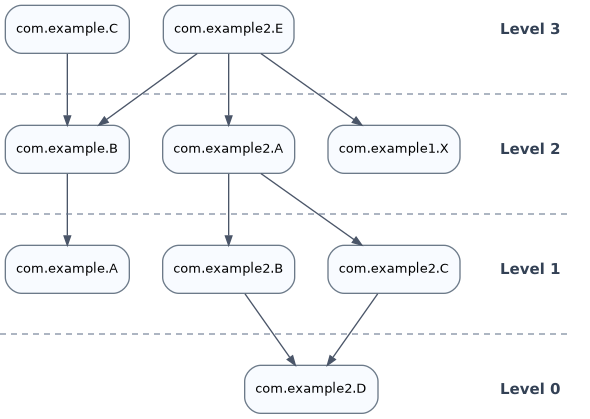
\includegraphics[width=0.75\textwidth]{figures/test-example-classgraph-acyclic-levels.png}
  \caption{Azyklisches Beispiel aus \texttt{test-example-1.0.0.jar}.}
  \label{fig:acyclic-levels}
\end{figure}

Die Pfeile zwischen den Boxen sind Abh\"angigkeiten von Klassen durch Aufruf
oder Nutzung. Im Beispiel nutzt \texttt{com.example.B} die Klasse
\texttt{com.example.A}, kurz $B \to A$. Die horizontalen Linien sind manuell
erg\"anzt und visualisieren die Ebenen der Schichtung. Level~0 bildet das
Fundament; h\"ohere Levels stehen f\"ur Elemente, die von darunterliegenden
Elementen abh\"angen.

Diese Art der Darstellung ist n\"utzlich und weit verbreitet. Als Visualisierung
realer Anwendungen hat sie aber drei praktische Probleme:

\begin{enumerate}
  \item Viele Pfeile machen die Grafik schon bei mittelgro\ss{}en Anwendungen
        un\"ubersichtlich.
  \item Die Paketstruktur ist \"uber mehrere Levels verteilt und bildet keine
        sichtbare Gruppierung.
  \item Bei zyklischen Abh\"angigkeiten muss der Zyklus f\"ur die
        Levelberechnung aufgebrochen werden, damit \"uberhaupt eine vertikale
        Ordnung entsteht. Der urspr\"ungliche Abh\"angigkeitsgraph bleibt
        unver\"andert; ver\"andert wird nur der daraus abgeleitete DAG
        (\emph{Directed Acyclic Graph}, ein gerichteter Graph ohne Zyklen), auf
        dem die Levels berechnet werden. Entscheidend ist deshalb, welche
        Kante f\"ur diese Berechnung ausgeklammert wird, denn genau diese
        Kante erscheint sp\"ater als Bruch der berechneten Ordnung.
\end{enumerate}

\section{S202 als hierarchische Schichtendarstellung}

Mit dem Open-Source-Werkzeug S202 versuchen wir, diese Probleme gezielt zu
adressieren. S202 ersetzt den flachen Klassengraphen nicht einfach durch eine
verbesserte Darstellung, sondern durch eine hierarchische
Architekturhypothese: Pakete bleiben als Container sichtbar, und innerhalb
jedes Containers werden Pakete oder Klassen nach ihren Abh\"angigkeiten
angeordnet.

Die Pfeile k\"onnen optional eingeblendet werden. Im Normalfall soll die
vertikale Ordnung aber bereits ohne Pfeile verst\"andlich machen, welche
Teile der Anwendung weiter oben liegen und welche als Fundament dienen.
Unerw\"unschte Abh\"angigkeiten fallen dadurch nicht als einzelne Linie in einem
gro\ss{}en Netz auf, sondern als Bruch in einer erwarteten Schichtenordnung.

Im Gegensatz zum flachen Klassengraphen sind die Levels bei S202 hierarchisch
durch die Paketstruktur gegliedert. Jedes Paket ordnet seine direkten Kinder,
also Subpakete oder Klassen, nach deren lokalen Abh\"angigkeiten. Die
Paketstruktur bleibt dadurch sichtbar, statt im Klassengraphen
auseinandergezogen zu werden.

\begin{figure}[H]
  \centering
  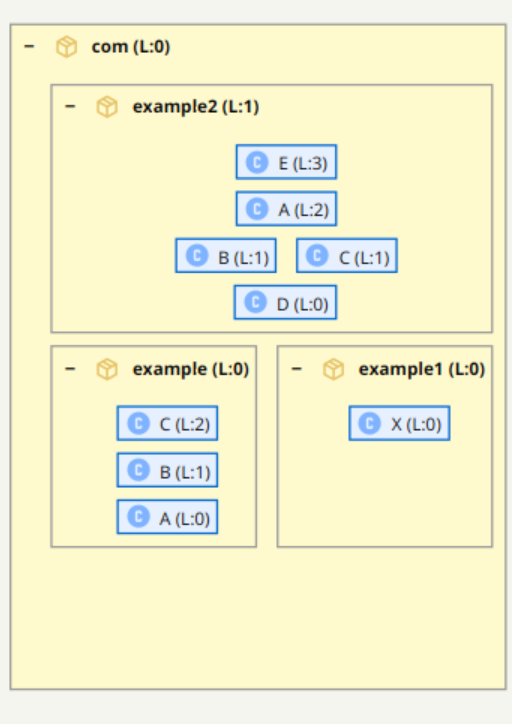
\includegraphics[width=0.55\textwidth]{figures/s202-dependencies-acyclic.png}
  \caption{S202-Darstellung des azyklischen Beispielausschnitts: Pakete
  bleiben als Container sichtbar, Klassen werden innerhalb ihres Containers
  geordnet, und Pfeile k\"onnen bei Bedarf eingeblendet werden.}
  \label{fig:s202-acyclic}
\end{figure}

Das Beispiel zeigt die Paketstruktur unterhalb des \"au\ss{}eren Pakets
\texttt{com}: \texttt{example}, \texttt{example1} und \texttt{example2} sind
Teilb\"aume dieses Containers. Im Teilbaum \texttt{example2} gibt es eine
nicht triviale innere Klassenstruktur; zugleich zeigt die \"ubergreifende Struktur, dass
\texttt{example2} von \texttt{example} und \texttt{example1} abh\"angt. Auf
Klassenebene gilt f\"ur \texttt{example2}: $E \to A \to (B \mid C) \to D$.
Die Darstellung abstrahiert dabei bewusst von einzelnen Kanten. Ob \texttt{A}
eine Abh\"angigkeit nach \texttt{B}, nach \texttt{C} oder nach beiden hat, ist
f\"ur die grobe Architekturansicht weniger wichtig als die Schichtung des
Pakets. Genau diese Abstraktion macht umfangreiche Beziehungsnetze noch lesbar.

Die Idee ist nicht neu. Das kommerzielle Produkt Structure101 hatte bereits
eine sehr \"ahnliche Darstellung. Es gibt jedoch keine offene Implementierung
und keine technische Dokumentation, die erkl\"art, wie man ein solches Layout
zuverl\"assig berechnet. S202 schlie\ss{}t diese L\"ucke als Open-Source-Werkzeug
unter der Apache-Lizenz.

Dieses Dokument beschreibt die typischen Fallstricke bei der Realisierung
eines solchen Layouts und zeigt eine L\"osung, mit der sich viele dieser
Probleme konzeptionell sauber eliminieren lassen.

\section{Typische Fehler bei der Berechnung von Schichten}

Die Abbildungen~\ref{fig:acyclic-levels} und~\ref{fig:s202-acyclic} zeigen
bewusst ein einfaches, azyklisches Beispiel. F\"ur diesen Fall ist die
Schichtung eindeutig: \texttt{E} steht \"uber \texttt{A}, \texttt{A} steht
\"uber \texttt{B} und \texttt{C}, und beide stehen \"uber \texttt{D}. Es gibt
keine R\"uckkopplung, deshalb muss keine Kante ausgew\"ahlt werden, die f\"ur
die Levelberechnung ignoriert wird.

In realen Anwendungen ist dieser Fall eher die Ausnahme. Sobald Klassen oder
Pakete zyklisch voneinander abh\"angen, reicht ein normaler Durchlauf \"uber
den Graphen nicht mehr aus. Genau dort beginnen die interessanten Fehler: Die
Darstellung sieht oft noch plausibel aus, aber die berechneten Ebenen sind
nicht mehr stabil oder nicht mehr fachlich erkl\"arbar.

In den folgenden Abschnitten spielt der Begriff SCC eine zentrale Rolle. Eine
SCC (\emph{Strongly Connected Component}, stark zusammenh\"angende Komponente)
ist eine Menge von Knoten, in der jeder Knoten jeden anderen
\"uber gerichtete Abh\"angigkeitspfade erreichen kann. In einem solchen Zyklus
k\"onnen nicht alle Abh\"angigkeiten gleichzeitig nach unten laufen.

Ein korrektes Schichtlayout muss deshalb gleichzeitig mehrere Anforderungen
erf\"ullen:

\begin{enumerate}
  \item Wenn $A \to B$ gilt, muss $A$ oberhalb von $B$ stehen.
  \item Pakete m\"ussen als Container sichtbar bleiben. Ein Paket darf nicht
        zuf\"allig verschoben werden, nur weil eine einzelne enthaltene Klasse
        ein hohes Klassenlevel hat.
  \item Klassen oder Pakete, die eine SCC bilden, m\"ussen explizit behandelt
        werden, weil in einem Zyklus nicht alle Kanten gleichzeitig nach unten
        laufen k\"onnen.
\end{enumerate}

Diese Anforderungen sind einzeln gut l\"osbar. Zusammen erzeugen sie aber ein
zirkul\"ares Abh\"angigkeitssystem zwischen den Ebenen der Berechnung selbst:
Klassenlevel beeinflussen sichtbare Positionen, Paketcontainer strukturieren
diese Positionen, und SCCs erzwingen Korrekturen an einer Ordnung, die man
ohne Zyklusbehandlung schon berechnet h\"atte. Genau daraus entstehen die
typischen Fehlermodi.

\subsection{Retroaktive Korrektur}

Retroaktive Korrektur bedeutet hier: Eine sp\"ater erkannte Struktur erzwingt
eine nachtr\"agliche \"Anderung an bereits berechneten Levels.

Ein naiver Algorithmus l\"auft \"uber die Klassen und vergibt direkt Level. Er
sieht zuerst Klasse \texttt{A}, setzt ihr Level und hebt damit auch das Paket
von \texttt{A} an. Sp\"ater findet er Klasse \texttt{B} und erkennt: \texttt{A}
und \texttt{B} geh\"oren zu derselben SCC und m\"ussen gemeinsam behandelt
werden. Jetzt m\"usste \texttt{A} korrigiert werden, und damit auch ihr Paket
und m\"oglicherweise weitere Pakete, die davon abh\"angen.

Das Problem ist nicht die Korrektur selbst. Das Problem ist, dass Teile des
Layouts zu diesem Zeitpunkt bereits als fertig behandelt wurden. Ein
Algorithmus, der Zyklenerkennung und Levelvergabe vermischt, muss r\"uckwirkend
an Stellen \"andern, die er eigentlich schon verlassen hat.

\subsection{Reihenfolgeabh\"angige Ergebnisse}

Klassen kommen aus Jars. Die Reihenfolge, in der ein Tool Klassen sieht, folgt
nicht der Architektur, sondern der Packreihenfolge des Jars, der Modulreihenfolge,
dem Build-Tool oder Details des Dateisystems. Wenn ein Algorithmus Zyklen
w\"ahrend dieser Traversierung nebenbei behandelt, h\"angt das Ergebnis von
dieser zuf\"alligen Reihenfolge ab.

Das ist gef\"ahrlich, weil der Fehler nicht sofort sichtbar sein muss. Die
Grafik kann weiterhin ungef\"ahr richtig aussehen. Trotzdem kann dieselbe
Codebasis je nach Build-Konfiguration andere Level bekommen.

\subsection{Vermischte Klassen- und Paketlevel}

Ein naheliegender Fehler ist, das Level eines Pakets aus dem h\"ochsten Level
seiner enthaltenen Klassen abzuleiten. Das klingt plausibel, vermischt aber
zwei verschiedene Fragen: Wo liegt eine Klasse im Klassengraphen, und wo liegt
ein Paket in der Architekturhypothese?

Ein Paket ist nicht deshalb architektonisch hoch, weil es zuf\"allig eine hoch
eingeordnete Klasse enth\"alt. Die zentrale Regel lautet:

\begin{quote}
  Paketlevel entstehen aus Paketabh\"angigkeiten, nicht aus der maximalen
  H\"ohe einzelner Klassen.
\end{quote}

Das klingt trivial, ist es aber nicht. Gerade weil Pakete Container f\"ur
Klassen sind, liegt es nahe, ihre Position aus den enthaltenen Klassen
abzuleiten. Genau dadurch vermischt man jedoch zwei Ebenen, die getrennt
bleiben m\"ussen. Erst wenn Paketlevel aus Paketabh\"angigkeiten entstehen,
bleiben Pakete stabile architektonische Einheiten. Sonst gen\"ugt eine einzige
Ausrei\ss{}er-Klasse, um das Paket auf die falsche Ebene zu heben~-- und damit
den Container unbrauchbar zu machen, der eigentlich Orientierung bieten soll.

Dieselbe Vermischung gibt es eine Ebene h\"oher. Wird das Level eines
Pakets aus einem Graphen berechnet, in den auch die Abh\"angigkeiten seiner
Unterpakete untereinander einflie\ss{}en, dann steigt ein Paket allein deshalb,
weil es innen tief geschichtet ist. Ein Paket, das alles enth\"alt, was es
benutzt, geh\"ort auf Level~0~-- gleichg\"ultig, wie seine Kinder zueinander
stehen. Die Regel lautet deshalb vollst\"andig: Das Level eines Elements
entsteht nur aus Abh\"angigkeiten, die sein eigenes Inneres verlassen.

\subsection{Der gro\ss{}e See}

Die formal saubere Antwort auf Zyklen lautet: Alle Elemente einer SCC bekommen
dasselbe Level. F\"ur kleine Zyklen ist das akzeptabel. In realen Systemen
k\"onnen SCCs aber sehr gro\ss{} werden. Dann landen Hunderte oder Tausende von
Klassen auf derselben Ebene. Die Schichtung verschwindet; \"ubrig bleibt ein
flacher Block.

Damit wird der Zyklus zwar korrekt erkannt, aber nicht mehr brauchbar
visualisiert. Ein Werkzeug muss gro\ss{}e SCCs daher aufbrechen k\"onnen.
Entscheidend ist, dass die geschnittenen Kanten nicht verschwinden. Sie m\"ussen
sichtbar bleiben, weil genau sie erkl\"aren, warum die berechnete Ordnung nur
als Architekturhypothese gilt.

\section{Zwei Arten von Zyklen}

S202 unterscheidet zwei grundlegend verschiedene Arten von Zyklen und macht
beide als getrennt schaltbare Overlays sichtbar:

\begin{description}
  \item[Klassenzyklen (rot)] Stark zusammenh\"angende Komponenten auf Klassenebene.
        Zwei oder mehr Klassen, die direkt oder transitiv voneinander abh\"angen,
        bilden einen solchen Zyklus. Klassenzyklen zeigen implementierungsebene
        Kopplung, die eine strikt lineare Ordnung einzelner Klassen verhindert.
        Sie werden mit dem Tarjan-Algorithmus auf dem Klassenabh\"angigkeitsgraphen
        erkannt.
  \item[Paketzyklen (orange)] Tangles innerhalb eines Containers. Ein
        Container ist ein Paket (oder die Wurzel); seine Kinder sind die direkt
        enthaltenen Klassen und Unterpakete. Zwei Kinder h\"angen voneinander
        ab, sobald irgendeine Klasse im Teilbaum des einen eine Klasse im
        Teilbaum des anderen benutzt. Bilden Kinder eines Containers auf diese
        Weise einen Zyklus und ist mindestens eines davon ein Paket, liegt ein
        Paketzyklus vor~-- unabh\"angig davon, welche konkreten Klassen daf\"ur
        verantwortlich sind. Paketzyklen zeigen Kopplung auf architektonischer
        Ebene: Die Paketstruktur selbst hat zirkul\"are Abh\"angigkeiten.
        Ein Zyklus, der nur aus Klassen desselben Pakets besteht, ist kein
        Paketzyklus; ihn zeigt das rote Overlay.
\end{description}

Der Unterschied ist wichtig, weil die beiden Arten verschiedene Fragen beantworten:

\begin{itemize}
  \item Ein \emph{Klassenzyklus} zeigt, welche konkreten Klassen entwirrt werden
        m\"ussen. Die Aufl\"osung erfordert oft das Verschieben einer Methode,
        das Extrahieren eines Interfaces oder das Umkehren einer Abh\"angigkeit
        zwischen zwei bestimmten Klassen.
  \item Ein \emph{Paketzyklus} zeigt, wo die Paketgrenzen selbst gebrochen sind.
        Die Aufl\"osung kann eine gr\"o\ss{}ere Umstrukturierung erfordern~--
        etwa das Zusammenf\"uhren zweier Pakete, das Einf\"uhren eines neuen oder
        die Neudefinition des Modulschnitts.
\end{itemize}

Ein Paketzyklus kann existieren, auch wenn kein einzelner Klassenzyklus sichtbar
ist~-- zum Beispiel wenn sich zwei Pakete \"uber verschiedene Klassen gegenseitig
aufrufen, die jeweils f\"ur sich azyklisch sind. Umgekehrt bedeutet ein
Klassenzyklus, der vollst\"andig innerhalb eines einzigen Pakets liegt, nicht
zwingend einen Paketzyklus.

Da die beiden Overlays verschiedene Fragen beantworten, h\"alt S202 sie als
unabh\"angige Schalter vor. Beide gleichzeitig zu aktivieren ist m\"oglich und
hilfreich, wenn man die Ursache eines architektonischen Problems sucht; jedes
Overlay ist aber auch allein aussagekr\"aftig: Das Paket-Zyklus-Overlay zeigt
die strukturelle Form des Problems, das Klassen-Zyklus-Overlay zeigt die
konkreten Kanten, die es verursachen.

\section{Der Container als Ordnungseinheit}

Die von S202 gew\"ahlte L\"osung besteht darin, Analyse, Ordnungsbildung und
Darstellung konsequent zu trennen. Der Klassengraph bleibt das Rohmodell der
tats\"achlichen Abh\"angigkeiten. Er wird nicht ver\"andert, nur weil f\"ur eine
Schichtendarstellung ein DAG ben\"otigt wird. Stattdessen erzeugt S202 aus
diesem Graphen zus\"atzliche Sichten: SCCs f\"ur die Zyklenerkennung, einen
gewichteten Geschwistergraphen je Container f\"ur die Ordnungsbildung und eine
hierarchische UI-Struktur f\"ur die Darstellung.

Mit Architekturhypothese ist dabei keine behauptete Soll-Architektur gemeint.
Gemeint ist eine aus den beobachteten Abh\"angigkeiten abgeleitete
Ist-Architektur: die Ordnung, die dem vorhandenen Code und seinen
Abh\"angigkeiten am engsten entspricht, ohne zu verbergen, wo diese Ordnung
durch Zyklen oder R\"uckkanten gebrochen wird.

Die Ordnungseinheit ist der Container. Jedes Paket ordnet seine direkten
Kinder~-- Klassen wie Unterpakete~-- ausschlie\ss{}lich nach den
Abh\"angigkeiten, die zwischen diesen Kindern verlaufen. Was innerhalb eines
Kindes geschieht, ist Sache dieses Kindes; was den Container verl\"asst, ist
Sache seines Elternpakets. Nach derselben Regel baut Structure101 seine
\emph{Levelized Structure Maps}. Sie ist der entscheidende Schritt: Eine
Klassenabh\"angigkeit wird genau einmal gewertet, n\"amlich in dem Container,
der beide Enden als Kinder verschiedener Teilb\"aume enth\"alt. Es gibt keine
globale Paketordnung, aus der die lokale abgeleitet w\"urde, und folglich auch
keine lokale Ordnung, die einer globalen widersprechen k\"onnte. Ein Paket
bleibt als Container stabil, weil nur seine Beziehungen zu seinen Geschwistern
seine Position bestimmen. Zugleich liefert die Container-Ordnung ein Kriterium,
um Back-Edges nicht beliebig auszuw\"ahlen, sondern als konkrete Verletzungen
der erwarteten Ordnung zu kennzeichnen.

Damit verschwinden die oben beschriebenen Fehlermodi nicht durch einen einzelnen
Algorithmustrick, sondern durch eine klare Zust\"andigkeit: Jeder Container
entscheidet f\"ur sich und endg\"ultig. Erst werden Abh\"angigkeiten analysiert,
dann wird je Container eine plausible Ordnung bestimmt, danach wird die
sichtbare Struktur aufgebaut, und zuletzt wird gepr\"uft, ob die Darstellung
ihre eigene Aussage einh\"alt.

\section{Von Klassenabh\"angigkeiten zur Container-Ordnung}

Der flache Klassengraph ist in S202 nicht das sichtbare Layoutmodell. Er ist
ein Analyseartefakt: Er dient dazu, konkrete Abh\"angigkeiten zu erfassen, SCCs
zu erkennen und jede Abh\"angigkeit dem Container zuzuordnen, der \"uber ihre
Richtung entscheidet. Die sichtbare S202-Grafik entsteht danach aus der
Paketstruktur und der Ordnung innerhalb jedes Containers.

F\"ur jede Klassenabh\"angigkeit $X \to Y$ bestimmt S202 den tiefsten Container,
der $X$ und $Y$ gemeinsam enth\"alt, und die beiden Kinder dieses Containers,
in deren Teilb\"aumen $X$ und $Y$ liegen. Die Abh\"angigkeit wird zur Kante
zwischen diesen beiden Geschwistern~-- und nur dort:

\begin{lstlisting}
com.a.X -> com.b.c.Y    Container com     Kante com.a   -> com.b
com.a.X -> com.a.Y      Container com.a   Kante com.a.X -> com.a.Y
com.a.X -> com.a.b.Y    Container com.a   Kante com.a.X -> com.a.b
\end{lstlisting}

Das Gewicht einer Geschwisterkante ist die Summe der Methodenaufrufe aller
Klassenabh\"angigkeiten, die auf sie abgebildet werden; eine Abh\"angigkeit
ohne Aufrufz\"ahlung tr\"agt ein Fallback-Gewicht von~1 bei. Es wird nichts
propagiert: Weder die Quell- noch die Zielseite wird entlang der Ahnenkette
vervielf\"altigt. Die Zahl der Kanten ist durch die Zahl der
Klassenabh\"angigkeiten beschr\"ankt, und jede Abh\"angigkeit hat genau eine
Stelle, an der \"uber ihre Richtung entschieden wird. Klassen und Pakete sind in
diesem Graphen gleichberechtigte Knoten; eine Klasse direkt im Paket und ein
Unterpaket desselben Pakets werden gegeneinander geordnet.

Zyklen in einem Geschwistergraphen sind die Tangles dieses Containers. Vor der
Levelberechnung muss der Graph azyklisch sein. Bilden Geschwister eine SCC,
bewertet S202 mit einem Rangma\ss{}, ob ein Geschwister eher andere nutzt oder
eher von ihnen genutzt wird:

\[
  rank(S) = \frac{out(S) - in(S)}{\max(1,\; out(S) + in(S))}
\]

$out(S)$ ist die Summe der Kantengewichte von $S$ zu anderen Mitgliedern
derselben SCC, $in(S)$ die Summe der Kantengewichte aus diesen Mitgliedern
nach $S$. Ein positiver Rang bedeutet: Das Element benutzt mehr, als es selbst
benutzt wird; es geh\"ort tendenziell nach oben. Ein negativer Rang bedeutet:
Das Element wird eher benutzt und geh\"ort tendenziell nach unten.

In einer SCC werden alle Kanten $S \to T$ geschnitten, f\"ur die
$rank(S) < rank(T)$ gilt~-- also alle Kanten, die gegen den
Abh\"angigkeitsstrom laufen. Es wird kein Schwellwert verwendet: Jede messbare
Rankdifferenz reicht als Begr\"undung f\"ur einen Schnitt. Sind alle Ranks
innerhalb einer SCC gleich, liefert die Topologie keine Richtungsinformation.
In diesem Fall werden alle internen Kanten entfernt, und die Levels der
betroffenen Knoten entstehen ausschlie\ss{}lich aus Abh\"angigkeiten au\ss{}erhalb
der ehemaligen SCC. Gibt es auch dort keine Abh\"angigkeiten, bleiben die
Knoten auf demselben Level~-- als echte Peers ohne begr\"undbare Ordnung.

Beide Schnittarten werden iterativ angewendet: Nach jedem Durchlauf werden die
SCCs neu bestimmt, und f\"ur verbleibende Rest-SCCs werden die Ranks \"uber
deren Mitglieder neu berechnet. Das Verfahren endet, wenn keine SCC mit
mindestens zwei Mitgliedern mehr existiert. Die Symmetrieerkennung beruht auf
dem Rankma\ss{}, nicht auf einem Gewichtsvergleich: Eine SCC, in der alle Kanten
dasselbe Gewicht tragen, ist nicht zwingend symmetrisch, weil unterschiedliche
Ein- und Ausgangsgrade trotz gleicher Gewichte verschiedene Ranks erzeugen.
Die geschnittenen Geschwisterkanten sind die \emph{Container-Back-Edges}.
Structure101 sucht an dieser Stelle eine m\"oglichst kleine Menge von
R\"uckkopplungskanten; der Rank-Schnitt ist daf\"ur ein deterministischer
Ersatz ohne Minimierungsanspruch. Er ist reihenfolgeunabh\"angig, weil alle
Elemente in sortierter Reihenfolge verarbeitet werden.

Nach dieser Zyklusbehandlung berechnet S202 die Levels auf dem resultierenden
DAG. Level~0 bilden die Geschwister, die keine anderen Geschwister benutzen.
Jedes andere Geschwister liegt eine Ebene \"uber dem h\"ochsten Geschwister, das
es direkt benutzt. Dadurch entsteht die transitive Schichtung: Aus $B \to A$
und $C \to B$ folgt $A$ auf Level~0, $B$ auf Level~1 und $C$ auf Level~2, auch
wenn keine direkte Kante $C \to A$ existiert.

Diese Regel~-- bekannt als \emph{Longest-Path-} oder \emph{ASAP-Levelisierung}~--
verankert jedes Element so tief wie m\"oglich, unmittelbar \"uber seiner tiefsten
Abh\"angigkeit. Sie deckt sich mit der Invariante, die Structure101 f\"ur seine
Levelized Structure Maps dokumentiert: Jedes Element h\"angt von mindestens einem
Element auf der unmittelbar darunterliegenden Ebene ab. Die Alternative, jedes
Element stattdessen b\"undig \emph{unter seinen Abnehmer} zu ziehen (ALAP), w\"urde
diese Invariante verletzen, da zwischen einem Element und seiner n\"achsten
Abh\"angigkeit eine L\"ucke entstehen k\"onnte.

Eine Folge ist bewusst in Kauf zu nehmen: Geschwister mit gleicher Rolle, aber
unterschiedlich tiefen Abh\"angigkeitsketten landen auf verschiedenen Levels.
Stehen etwa mehrere Adapter \"uber derselben Anwendungsschicht, einer von ihnen
aber zus\"atzlich \"uber einem gemeinsamen Hilfspaket, so liegt dieser eine Ebene
h\"oher als die \"ubrigen~-- die Levelisierung misst Abh\"angigkeitstiefe, nicht
architektonische Rolle.

Das so berechnete \emph{localLevel} ist die Architekturhypothese. Es
bestimmt die Position jedes Elements innerhalb seines Containers, und die
Kette der localLevels von der Wurzel bis zum Element ist die Ordnung, gegen
die Verletzungen gemessen werden. Es ist bewusst lokal: Es vergleicht nur
Geschwister.

Daneben f\"uhrt S202 f\"ur jedes Element ein globales \emph{architectureLevel}.
Es misst, wie tief die Abh\"angigkeitskette unter einem Element tats\"achlich
ist, und ist damit ein Ma\ss{} f\"ur dessen Komplexit\"at; die H\"ohe in der
3D-Darstellung und der Ring der hexagonalen Sicht beruhen darauf. Das
\emph{architectureLevel} einer Klasse ist ihre Longest-Path-Tiefe im
Klassengraphen. Ausgeklammert werden dabei nur die \emph{Level-Schnitte}:
Back-Edges, die innerhalb eines Klassenzyklus liegen. Eine Back-Edge, die
lediglich gegen die Ordnung zweier Pakete l\"auft, ohne einen Klassenzyklus zu
schlie\ss{}en, ist eine echte azyklische Abh\"angigkeit und z\"ahlt weiter. Das
\emph{architectureLevel} eines Pakets folgt derselben Regel eine Ebene h\"oher:
Es ist seine Longest-Path-Tiefe in einem Paketgraphen, in dem $P$ von $Q$
abh\"angt, wenn eine Nicht-Back-Edge aus dem Teilbaum von $P$ in den Teilbaum
von $Q$ f\"uhrt und keines der beiden Pakete das andere enth\"alt. Beide Graphen
sind konstruktionsbedingt azyklisch. Ein Paket wird so nie von seinem eigenen
Inneren angehoben: Wer alles enth\"alt, was er benutzt, steht auf Level~0. Das
globale Level beeinflusst weder das Layout noch die Verletzungserkennung.

\section{Vom Klassenzyklus zur Back-Edge}

Abbildung~\ref{fig:cyclic-class} zeigt ein zyklisches Beispiel aus dem
Example-Jar als klassischen Klassengraphen. Die beiden Teilgraphen f\"ur Notification und
Payment enthalten jeweils R\"uckkopplungen.

\begin{figure}[H]
  \centering
  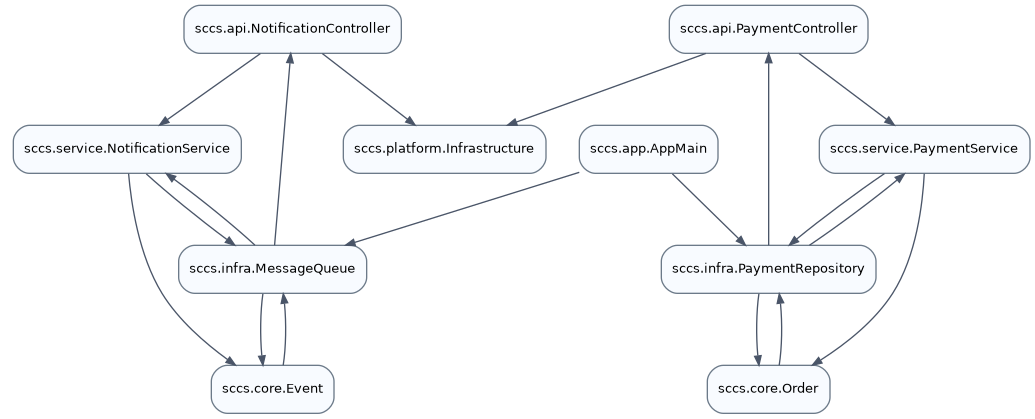
\includegraphics[width=0.9\textwidth]{figures/test-example-classgraph-cyclic.png}
  \caption{Zyklisches Beispiel aus \texttt{test-example-1.0.0.jar}. In jedem
  Zyklus muss mindestens eine Kante f\"ur die Levelberechnung geschnitten werden.}
  \label{fig:cyclic-class}
\end{figure}

Die markierten zyklischen Bereiche sind zwei nicht-triviale SCCs: eine
Notification-SCC mit \texttt{NotificationController}, \texttt{NotificationService},
\texttt{MessageQueue} und \texttt{Event}, sowie eine Payment-SCC mit
\texttt{PaymentController}, \texttt{PaymentService}, \texttt{PaymentRepository}
und \texttt{Order}. Das etablierte Verfahren zur Ermittlung solcher Komponenten
ist der Tarjan-Algorithmus.

Damit stellt der Klassengraph im Zyklusfall die technische Frage: Welche Kante
muss man ignorieren, damit aus der SCC wieder ein berechenbarer DAG f\"ur die
Levelbildung wird? Der Klassengraph allein liefert daf\"ur aber kein fachliches
Kriterium. Die Container-Ordnung liefert es: Eine Klassenabh\"angigkeit ist
genau dann eine Back-Edge, wenn ihre Projektion in ihrem Container eine
geschnittene Geschwisterkante ist.

Ein Klassenzyklus, der innerhalb eines Pakets liegt, wird in diesem Paket
geschnitten~-- dort sind die Klassen selbst die Geschwister. Ein Klassenzyklus,
der mehrere Pakete durchl\"auft, erscheint im gemeinsamen Elterncontainer als
Tangle zwischen Paketen und wird dort geschnitten; innerhalb der beteiligten
Pakete z\"ahlen nur noch die Kanten, deren beide Enden darin liegen. Die
retroaktive Korrektur aus dem Fehlerkatalog kann so nicht entstehen: Kein
Container muss eine Entscheidung eines anderen revidieren.

Daraus folgt eine Eigenschaft, die sich beweisen l\"asst: Jeder Klassenzyklus
enth\"alt mindestens eine Back-Edge. Im tiefsten Container, der alle Klassen
des Zyklus enth\"alt, bildet er sich auf einen Zyklus zwischen Geschwistern ab,
und dort wurde mindestens eine Kante geschnitten. F\"ur das globale
Klassenlevel gen\"ugt es deshalb, die Back-Edges innerhalb von Klassenzyklen
auszuklammern~-- die \emph{Level-Schnitte}. Der Klassengraph ist danach
azyklisch; die Levelberechnung braucht keine weitere Zyklusbehandlung und keine
Sonderf\"alle.

Back-Edges au\ss{}erhalb von Klassenzyklen bleiben dagegen in der
Levelberechnung. Zwei Pakete k\"onnen einander \"uber verschiedene Klassen
benutzen, ohne dass ein Klassenzyklus entsteht. Die Kante gegen die
Paketordnung ist dann eine Verletzung im Bild, aber weiterhin Teil der
tats\"achlichen Abh\"angigkeitstiefe ihrer Klasse.

Alle Back-Edges werden als \emph{classBackEdge}-Befunde erfasst und bleiben als
gestrichelte Verletzungskanten sichtbar.

\begin{figure}[H]
  \centering
  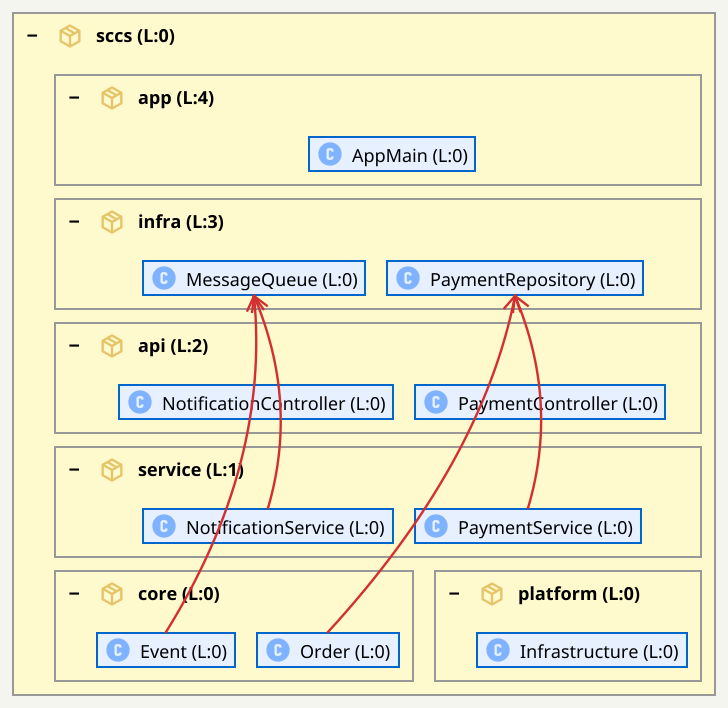
\includegraphics[width=0.6\textwidth]{figures/s202-dependencies-cyclic.png}
  \caption{Zyklisches Beispiel in der S202-Darstellung. Die gestrichelten Kanten sind Verletzungen:
  Sie laufen gegen die berechnete Container-Ordnung und bleiben als sichtbarer
  Befund der Architekturhypothese erhalten. Alle vier gestrichelten Kanten sind
  Back-Edges: Projektionen der im Container \texttt{sccs} geschnittenen
  Geschwisterkanten \texttt{core}$\to$\texttt{infra} und
  \texttt{service}$\to$\texttt{infra}.}
  \label{fig:s202-cyclic}
\end{figure}

Die Begriffe Back-Edge und Verletzung beschreiben unterschiedliche Rollen
derselben Kanten:

\begin{description}
  \item[Back-Edge] Eine Klassenabh\"angigkeit, deren Projektion in ihrem
        Container beim Aufbrechen eines Tangles geschnitten wurde. Sie geh\"ort
        zur Zyklusbehandlung. Liegt sie zus\"atzlich in einem Klassenzyklus,
        ist sie ein Level-Schnitt und wird f\"ur das globale Klassenlevel
        ausgeklammert.
  \item[Verletzung] Eine konkrete Abh\"angigkeit, die nach der berechneten
        Ordnung nach oben l\"auft. Ma\ss{}geblich ist dabei die
        \emph{geschachtelte} Ordnung, nicht ein flaches globales Level: Verglichen
        wird die \emph{localLevel}-Kette beider Endpunkte vom \"au\ss{}ersten
        gemeinsamen Container abw\"arts; die Richtung entscheidet der erste
        Container, in dem sie sich unterscheiden (im Code \emph{visual rank}
        genannt). Jede Verletzung ist eine Back-Edge, denn au\ss{}erhalb der
        geschnittenen Kanten laufen alle Geschwisterkanten nach unten.
        Umgekehrt l\"auft eine Back-Edge nach oben oder seitw\"arts; nur wenn
        innerhalb eines Tangles ein zweiter Pfad die Richtung ohnehin festlegt,
        kann eine geschnittene Kante am Ende nach unten zeigen und ist dann
        keine sichtbare Verletzung. Begrifflich bleibt eine Verletzung die
        sichtbare Ordnungsabweichung, w\"ahrend eine Back-Edge die Rolle der
        Kante in der Zyklusbehandlung beschreibt.
\end{description}

S202 versteckt den Zyklus daher nicht. Als Back-Edges klassifizierte Kanten
bleiben als Verletzungen sichtbar, weil sie erkl\"aren, warum die
Container-Ordnung nicht vollst\"andig zu den konkreten Klassenabh\"angigkeiten
passt. Dadurch wird die Abweichung nachvollziehbar statt beliebig.

\section{Redundante Pr\"ufung der Konsistenz}

Die bisher beschriebenen Schritte zeigen bereits, warum die Umsetzung
fehleranf\"allig ist. Es reicht nicht, einzelne Algorithmen isoliert mit Unit
Tests abzusichern. Viele Fehler entstehen erst durch das Zusammenspiel der
Daten: konkrete Klassenabh\"angigkeiten, Paketstruktur, SCCs, aggregierte
Paketgewichte und lokale Darstellungspositionen beeinflussen sich gegenseitig.

S202 pr\"uft deshalb nicht nur einzelne Rechenschritte. Nachdem die komplette
Pipeline gelaufen ist, wird das fertige Ergebnis redundant gegen
Konsistenzregeln gepr\"uft. Diese Regeln berechnen das Layout nicht neu und
korrigieren auch nichts. Sie lesen nur das Ergebnis und fragen: Ist die
erzeugte Darstellung in sich stimmig?

Die Pr\"ufung besteht aus f\"unf Regeln:

\begin{enumerate}
  \item \textbf{Klassengraph:} F\"ur jede Klassenabh\"angigkeit $A \to B$, die
        kein Level-Schnitt ist, steht $A$ auf einem h\"oheren Level als $B$,
        und jeder Level-Schnitt ist eine Back-Edge. Es gibt keine weiteren
        Ausnahmen, weil der Klassengraph ohne Level-Schnitte azyklisch ist.
  \item \textbf{Container:} In jedem Container l\"auft jede nicht geschnittene
        Geschwisterkante von einem h\"oheren zu einem niedrigeren
        \emph{localLevel}. Das ist das Versprechen der Darstellung selbst.
  \item \textbf{Back-Edges nur in Tangles:} Jede geschnittene Geschwisterkante
        verbindet zwei Mitglieder desselben Container-Tangles. Au\ss{}erhalb von
        Zyklen wird nichts geschnitten.
  \item \textbf{Paketgraph:} F\"ur jede Nicht-Back-Edge zwischen Klassen zweier
        Pakete, die einander nicht enthalten, liegt das Quellpaket \"uber dem
        Zielpaket.
  \item \textbf{Sichtbare Darstellung:} Jede Abh\"angigkeit, die in der
        geschachtelten Ordnung nach oben l\"auft, ist eine Back-Edge. Die
        Darstellung zeigt keine Verletzung, die das Modell nicht kennt.
\end{enumerate}

Diese Konsistenzregeln sind keine zus\"atzliche Optimierung und kein zweiter
Layoutalgorithmus. Sie sind ein unabh\"angiger Plausibilit\"atscheck nach
Abschluss der Berechnung. Genau dadurch finden sie Fehler, die in normalen
Unit Tests leicht fehlen: eine Kante wurde beim Layout stillschweigend
geschnitten, ohne als Back-Edge zu gelten; eine Back-Edge liegt au\ss{}erhalb
jedes Tangles; eine normale Kante l\"auft nach oben. Genau der erste dieser
Fehler blieb in einer fr\"uheren Fassung von S202 lange unentdeckt, weil die
Ordnung aus einem globalen Paketgraphen und die Position aus einem lokalen
Geschwistergraphen stammten und niemand pr\"ufte, ob beide \"ubereinstimmen.

Der entscheidende Punkt ist Redundanz. Die Pipeline erzeugt die Darstellung.
Die Regeln pr\"ufen anschlie\ss{}end, ob diese Darstellung ihre eigene Aussage
einh\"alt. Damit wird aus einer reinen Grafik ein \"uberpr\"ufbares Modell.

\section{Von der Visualisierung zur Aktion}

Eine berechnete Architekturhypothese ist besonders dann n\"utzlich, wenn sie
nicht nur einen Zustand beschreibt, sondern Ver\"anderung planbar macht. S202
enth\"alt daf\"ur eine What-If-Analyse: Klassen und Pakete k\"onnen per Drag
and Drop in der Darstellung verschoben werden. Das Modell wird dadurch nicht
sofort refaktoriert; stattdessen berechnet das Werkzeug, welche Abh\"angigkeiten
in der neuen Anordnung nach oben laufen w\"urden.

Die Verletzungen aktualisieren sich nach jeder Verschiebung. Dadurch wird
sichtbar, ob eine geplante Umordnung die Architektur konsistenter macht oder
neue Probleme erzeugt. Das ist vor allem in Situationen wichtig, in denen das
Werkzeug keine eindeutige Ordnung mehr findet: gro\ss{}e SCCs, symmetrische
Paketabh\"angigkeiten oder historisch gewachsene Kopplungen lassen sich nicht
immer automatisch sinnvoll aufl\"osen.

\begin{figure}[H]
  \centering
  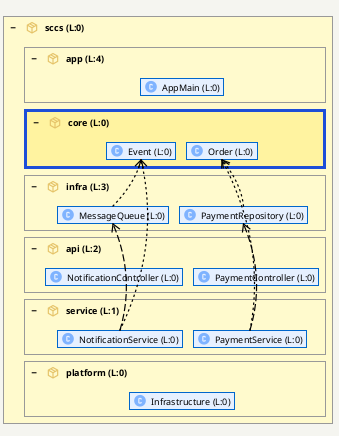
\includegraphics[width=0.45\textwidth]{figures/whatif-core-over-infra.png}
  \caption{What-If-Verschiebung: Das Paket \texttt{core} wird aus Level~0
  zwischen Level~3 und Level~4 verschoben. Dadurch entstehen sechs
  Verletzungen, weil bestehende Abh\"angigkeiten nun gegen die gew\"ahlte
  Anordnung laufen.}
  \label{fig:whatif-core-over-infra}
\end{figure}

Abbildung~\ref{fig:whatif-core-over-infra} zeigt genau diese Arbeitsweise:
Die manuelle Anordnung entspricht nicht mehr der aus den Abh\"angigkeiten
berechneten Ordnung. Sie kann trotzdem eine gew\"unschte Zielarchitektur
ausdr\"ucken, etwa wenn \texttt{core} fachlich oberhalb der Infrastruktur
liegen soll. S202 behandelt diese Entscheidung deshalb nicht als Fehler der
Darstellung, sondern macht ihre Kosten sichtbar: In diesem Fall m\"ussten sechs
konkrete Beziehungen refaktoriert oder entkoppelt werden, damit die
Abh\"angigkeiten wieder zur gew\"ahlten Schichtung passen.

Erg\"anzend dazu gibt es eine manuelle CUT-Logik. Back-Edges k\"onnen gezielt
als geplante Schnitte markiert werden, und das Werkzeug kann anschlie\ss{}end
pr\"ufen, ob diese Schnitte die betroffene SCC tats\"achlich aufl\"osen. Der
Benutzer sieht nicht nur, welche Kante als Bruch der Ordnung plausibel w\"are,
sondern kann die Wirkung dieses Schnitts auf den Zyklus \"uberpr\"ufen.

Diese CUT-Logik arbeitet feiner als die sichtbare Klassen- oder Paketkante.
Geschnitten wird auf Methodenaufrufebene: Nicht zwingend die gesamte Beziehung
zwischen zwei Klassen verschwindet, sondern der konkrete Methodenaufruf, der
die zyklische Abh\"angigkeit verursacht. Dadurch passt das Feature besser zur
praktischen Refactoring-Arbeit, weil ein Zyklus oft durch wenige konkrete
Aufrufe entsteht, nicht durch die komplette fachliche Beziehung zweier Klassen.

\section{Umsetzung auf konzeptioneller Ebene}

Die Umsetzung trennt die Berechnung bewusst in mehrere Phasen. Entscheidend
ist, dass keine Phase eine sichtbare Position festlegt, bevor die Informationen
vorliegen, die diese Position begr\"unden.

\begin{enumerate}
  \item \textbf{Klassengraph aufbauen:} Aus dem Bytecode wird ein gerichteter
        Klassengraph erzeugt. Dieser Graph bleibt das fachliche Rohmodell der
        Analyse. In die Ordnungsberechnung gehen nur Kanten ein, die mindestens
        eine Beziehung der Art \texttt{extends}, \texttt{implements},
        \texttt{imports}, \texttt{instantiates} oder \texttt{calls} tragen;
        reine Typreferenzen (Feldtypen, Parameter- und R\"uckgabetypen, Casts)
        bleiben im Rohmodell erhalten, werden aber nicht gewertet.
  \item \textbf{SCCs erkennen:} Auf dem Klassengraphen werden stark
        zusammenh\"angende Komponenten mittels Tarjan ermittelt. Das Ergebnis
        ist noch kein Layout, sondern die Information, welche Klassen azyklisch
        einordenbar sind und welche zu Zyklen geh\"oren (rotes Overlay).
  \item \textbf{Container ordnen:} Jede Klassenabh\"angigkeit wird auf die
        beiden Kinder des tiefsten gemeinsamen Containers projiziert und dort
        als gewichtete Geschwisterkante gez\"ahlt. Je Container werden die SCCs
        des Geschwistergraphen als Tangles erfasst (orangenes Overlay), mit dem
        Rank-Schnitt aufgel\"ost und die verbleibende Ordnung per Longest-Path
        in ein \emph{localLevel} je Kind \"ubersetzt. Die geschnittenen
        Geschwisterkanten sind die Container-Back-Edges.
  \item \textbf{Klassen-Back-Edges ableiten:} Eine Klassenabh\"angigkeit ist
        eine Back-Edge, wenn ihre Projektion geschnitten wurde. Sie bleibt als
        \emph{classBackEdge}-Befund erhalten und als gestrichelte
        Verletzungskante sichtbar.
  \item \textbf{Globale Levels berechnen:} Das \emph{architectureLevel}
        von Klassen entsteht per Longest-Path auf dem Klassengraphen ohne die
        Level-Schnitte~-- die Back-Edges innerhalb von Klassenzyklen~--, das
        von Paketen auf dem Paketgraphen aus Nicht-Back-Edges zwischen
        verschiedenen Teilb\"aumen. Beide Graphen sind konstruktionsbedingt
        azyklisch.
  \item \textbf{Konsistenz pr\"ufen:} Zum Schluss wird die fertige Darstellung
        redundant gegen die f\"unf Konsistenzregeln gepr\"uft.
\end{enumerate}

Kurz gefasst:

\begin{lstlisting}
Bytecode -> Klassengraph -> Klassen-SCCs (rotes Overlay)
         -> je Container: Geschwistergraph -> Tangles (orangenes Overlay)
                          -> Rank-Schnitt (Back-Edges) -> localLevel
         -> Klassen-Back-Edges -> Level-Schnitte
         -> architectureLevel (Klassen, Pakete)
         -> Konsistenzregeln
\end{lstlisting}

\section{Fazit}

S202 berechnet aus den bestehenden Abh\"angigkeiten die plausibelste Hypothese
der Ist-Architektur. Das Ergebnis ist eine \"uberpr\"ufbare hierarchische
Schichtendarstellung: Klassenabh\"angigkeiten liefern den Graphen, jeder
Container ordnet seine Kinder nach genau diesen Abh\"angigkeiten, Back-Edges
machen notwendige Br\"uche sichtbar, und Konsistenzregeln pr\"ufen, ob die
fertige Darstellung ihre eigene Aussage einh\"alt.

Eine wichtige Entwurfsentscheidung ist die explizite Trennung zweier
Zyklus-Arten. Klassenzyklen und Paketzyklen werden unabh\"angig voneinander
erkannt, als getrennte Befunde gespeichert und \"uber separate Schalter in der
Benutzeroberfl\"ache sichtbar gemacht. Klassenzyklen (rot) zeigen, welche
konkreten Klassen zyklische Abh\"angigkeitsketten bilden; Paketzyklen (orange)
zeigen, welche Pakete auf architektonischer Ebene gegenseitig abh\"angen. Da
beide Ansichten gleichzeitig verf\"ugbar sind, kann das Werkzeug zwei
verschiedene Fragen gleichzeitig beantworten: \emph{Wo} in der Paketstruktur
liegt die zirkul\"are Kopplung, und \emph{welche konkreten Klassenabh\"angigkeiten}
verursachen sie.

Der wichtigste Beitrag liegt deshalb nicht in einer optisch verbesserten
Grafik, sondern in der Verbindung von Darstellung, Erkl\"arung und
Ver\"anderbarkeit. Die Schichtung zeigt eine m\"ogliche Ordnung. Die markierten
Befunde erkl\"aren, wo diese Ordnung durch konkrete Abh\"angigkeiten gebrochen
wird. What-If-Verschiebungen und manuelle CUTs machen sichtbar, welche
Refactorings diese Br\"uche reduzieren oder Zyklen tats\"achlich aufl\"osen
k\"onnen.

Damit ist die Visualisierung mehr als ein Layout. Sie ist ein erkl\"arbares
Arbeitsmodell: Jede Position und jede hervorgehobene Kante muss auf eine
nachvollziehbare Entscheidung in der Berechnung zur\"uckf\"uhrbar sein, und
jede geplante \"Anderung kann gegen dieselbe Ordnung gepr\"uft werden.

\end{document}
